\documentclass[11pt,aspectratio=169]{beamer}
\usetheme{Copenhagen}

\AtBeginSection[]{
  \begin{frame}
  \vfill
  \centering
  \begin{beamercolorbox}[sep=8pt,center,shadow=true,rounded=true]{title}
    \usebeamerfont{title}\insertsectionhead\par%
  \end{beamercolorbox}
  \vfill
  \end{frame}
}

\usepackage{amsmath}
\usepackage{amssymb}
\usepackage{bm}
\usepackage{amsthm}
\usepackage{enumerate}
\usepackage{graphicx}
\usepackage{psfrag}
\usepackage{color}
\usepackage{url}
\usepackage{listings}
\usepackage{xcolor}
\usepackage{tikz}
% \usetikzlibrary{positioning}
% \tikzset{main node/.style={circle,fill=gray!20,draw,minimum size=.5cm,inner sep=0pt},}

% \definecolor{codegreen}{rgb}{0,0.5,0}
% \definecolor{codewhite}{rgb}{1,1,1}
% \definecolor{codegray}{rgb}{0.5,0.5,0.5}
% \definecolor{codepurple}{rgb}{0.58,0,0.82}
% \definecolor{codeblack}{rgb}{0,0,0}
% \definecolor{codeorange}{rgb}{0.8,0.4,0}

% \lstdefinestyle{mystyle}{
    % backgroundcolor=\color{codewhite},   
    % commentstyle=\color{codegray},
    % keywordstyle=\color{codegreen},
    % numberstyle=\color{codegray},
    % stringstyle=\color{codeorange},
    % basicstyle=\ttfamily ,
    % breakatwhitespace=false,         
    % breaklines=true,                 
    % captionpos=b,                    
    % keepspaces=true,                 
    % numbers=left,                    
    % numbersep=5pt,                  
    % showspaces=false,                
    % showstringspaces=false,
    % showtabs=false,                  
    % tabsize=4
% }
% \lstset{style=mystyle}


% \setlength{\hoffset}{-1in}
% \addtolength{\textwidth}{1.5in}
% \setlength{\voffset}{-1in}
% \addtolength{\textheight}{1.5in}
\newcommand{\be}{\begin{enumerate}}
\newcommand{\ee}{\end{enumerate}}
\newcommand{\BigO}[1]{\ensuremath\mathcal{O}\left(#1\right)}
\newcommand{\il}[1]{\lstinline!#1!}
\newcommand{\gnorm}[1]{\left|\left|#1\right|\right|}
\newcommand{\abs}[1]{\left|#1\right|}
\newcommand{\parens}[1]{\left(#1\right)}
\newcommand{\bracks}[1]{\left\{#1\right\}}
\newcommand{\sqbracks}[1]{\left[#1\right]}
\newcommand{\vep}{\varepsilon}
\newcommand{\ceiling}[1]{\left\lceil#1\right\rceil}
\newcommand{\R}{\mathbb{R}}
\newcommand{\N}{\mathbb{N}}
\newcommand{\Z}{\mathbb{Z}}
\newcommand{\distrib}[2]{\text{#1}\left(#2\right)}
\newcommand{\dd}[1]{\frac{d}{d#1}}
\newcommand{\abracks}[1]{\left< #1\right>}

\title{A study on quantifying effective training of DLDMD}
\author{Joseph A.G. Diaz}
\institute{Master of Science in Applied Mathematics\\ 
           with a Concentration in Dynamical Systems,\\
           San Diego State University}
\date{\today}

\begin{document}

    \frame{\titlepage}

    \begin{frame}
        \frametitle{Introduction}

        In the study of dynamical systems a central problem is how to derive models 
        from measured data to facilitate the prediction of future states. The data-driven
        method Dynamic Mode Decomposition and it's extensions offer a compelling avenue
        in the problem of prediction from time-series data.

        The marriage of these methods with Machine Learning and Neural Networks allows for
        the leveraging the power of these tools in the space. 

        If standard metrics of model training are unavailable, 
    
    \end{frame}

    \begin{frame}
        \frametitle{Introduction - The Network}
        Example of DLDMD newtork with $N_S = 2,\ N_O = 4,$ and $N_L = 3$ where every
        hidden layer has 16 neurons.
        \begin{figure}
            \centering
            \begin{minipage}{.5\textwidth}
                $$\mathcal{E}$$
                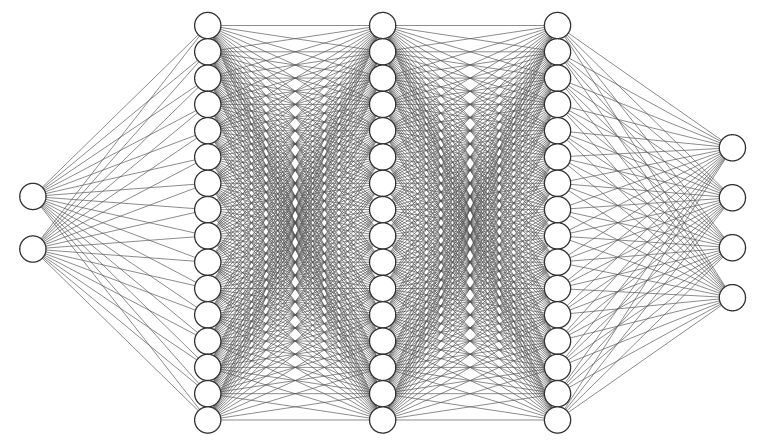
\includegraphics[width=\textwidth]{../Figures/Encoder.png}
            \end{minipage}%
            \begin{minipage}{.5\textwidth}
                $$\mathcal{D}$$
                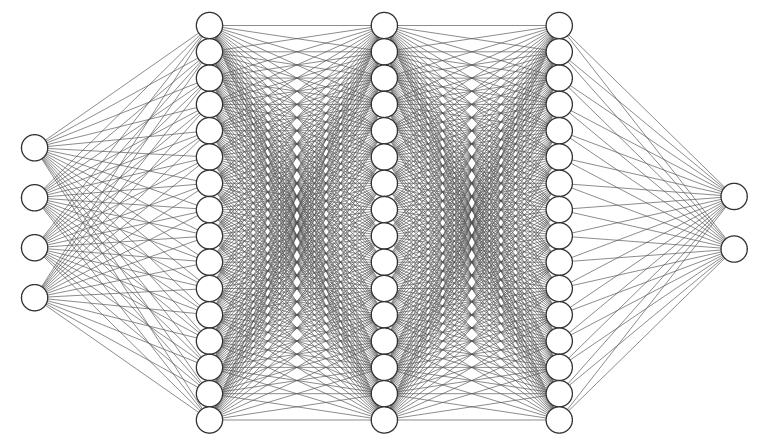
\includegraphics[width=\textwidth]{../Figures/Decoder.png}
            \end{minipage}
        \end{figure}
    \end{frame}

    \begin{frame}
        \frametitle{Kullback-Leibler Divergence - Entropy}
        \begin{figure}
            \centering
            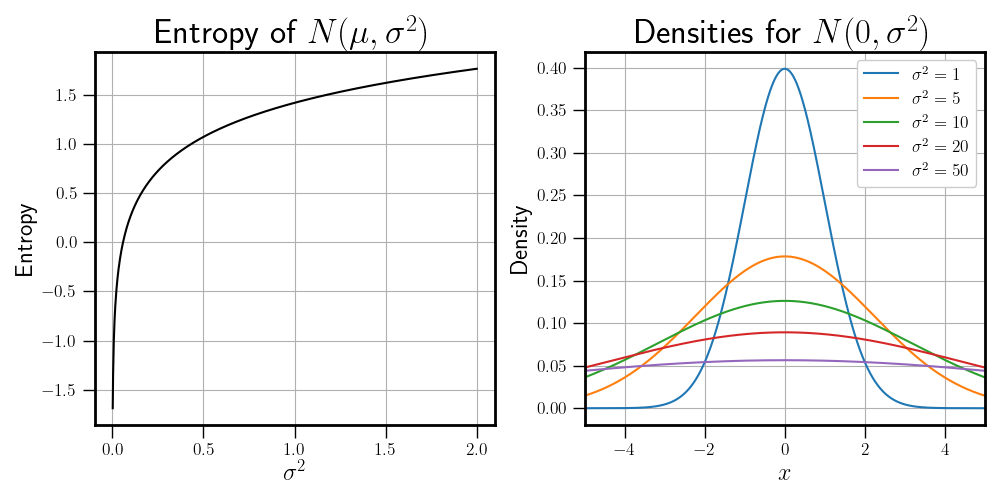
\includegraphics[width=\textwidth]{../Figures/entropy_densities_example.png}
        \end{figure}
    \end{frame}

    \begin{frame}
        \frametitle{Kullback-Leibler Divergence - normal distribution example}
        \begin{figure}
            \centering
            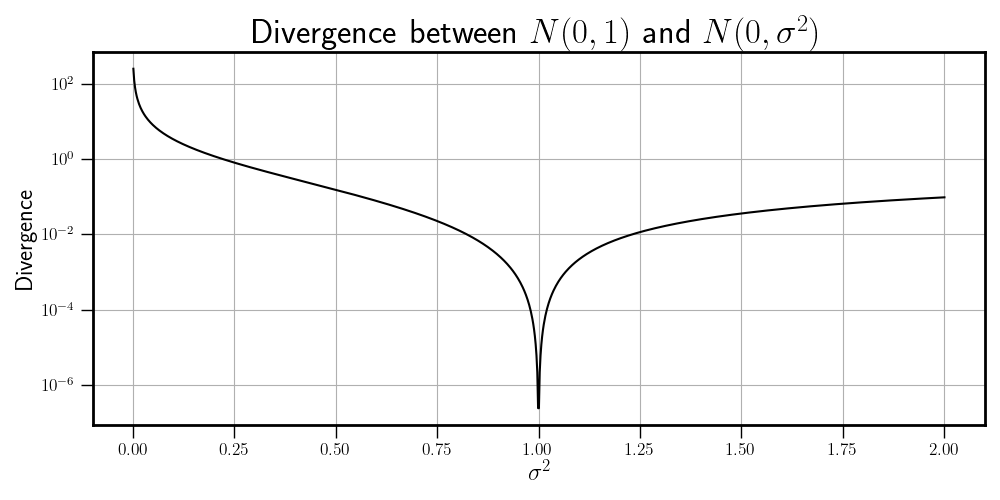
\includegraphics[width=\textwidth]{../Figures/divergence_example.png}
        \end{figure}
    \end{frame}

    \begin{frame}
        \frametitle{Kullback-Leibler Divergence - KDE example}
        \begin{figure}
            \centering
            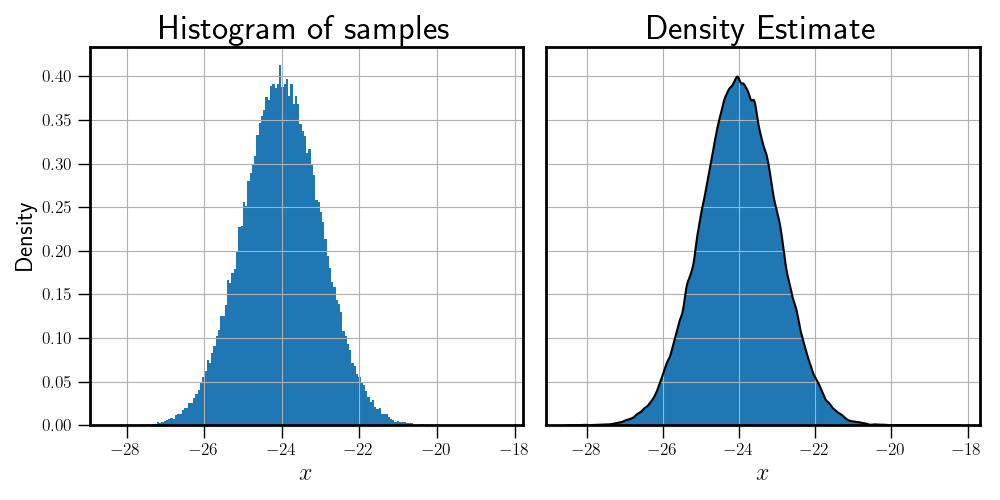
\includegraphics[width=\textwidth]{../Figures/kde_example.png}
        \end{figure}
    \end{frame}

    \begin{frame}
        \frametitle{Kullback-Leibler Divergence - Example fitting}
        \begin{figure}
            \centering
            \includegraphics[width=\textwidth]{"Z:/ML_models/DLDMD-newest/examples/van_der_pol/trained_models/van_der_pol_07_2022-07-17-1837/div_plot_linear_enc_1"}
        \end{figure}
    \end{frame}

    \begin{frame}
        \frametitle{Results - Duffing}
        \begin{figure}
            \centering
            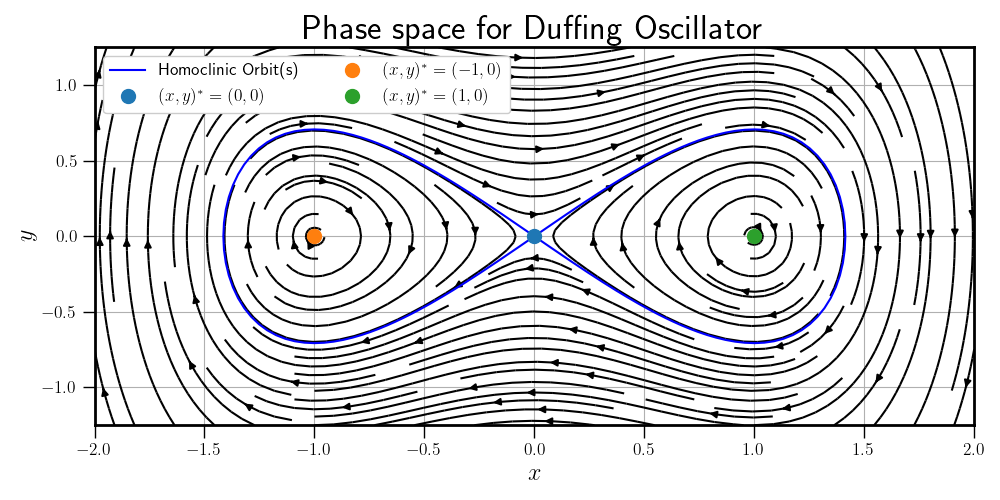
\includegraphics[width=\textwidth]{../Figures/duffing_phase_space.png}
        \end{figure}
    \end{frame}

    \begin{frame}
        \frametitle{Results - Duffing loss curves and phase space}
        \begin{figure}
            \centering
            \begin{minipage}{.5\textwidth}
                \includegraphics[width=\textwidth]{"Z:/ML_models/DLDMD-newest/examples/duffing/loss_plots_square.png"}
            \end{minipage}%
            \begin{minipage}{.5\textwidth}
                \includegraphics[width=\textwidth]{"Z:/ML_models/DLDMD-newest/examples/duffing/experiment_trajectories.png"}
            \end{minipage}
        \end{figure}
    \end{frame}
    
    \begin{frame}
        \frametitle{Results - Duffing linear fit slopes}
        \begin{figure}
            \centering
            \begin{minipage}{.3333\textwidth}
                \includegraphics[width=\textwidth]{"Z:/ML_models/DLDMD-newest/examples/duffing/slope_linear_fit_enc_in_square.png"}
                \includegraphics[width=\textwidth]{"Z:/ML_models/DLDMD-newest/examples/duffing/slope_linear_fit_enc_2_square.png"}
                \includegraphics[width=\textwidth]{"Z:/ML_models/DLDMD-newest/examples/duffing/slope_linear_fit_dec_0_square.png"}
            \end{minipage}%
            \begin{minipage}{.3333\textwidth}
                \includegraphics[width=\textwidth]{"Z:/ML_models/DLDMD-newest/examples/duffing/slope_linear_fit_enc_0_square.png"}
                \includegraphics[width=\textwidth]{"Z:/ML_models/DLDMD-newest/examples/duffing/slope_linear_fit_enc_out_square.png"}
                \includegraphics[width=\textwidth]{"Z:/ML_models/DLDMD-newest/examples/duffing/slope_linear_fit_dec_1_square.png"}
            \end{minipage}%
            \begin{minipage}{.3333\textwidth}
                \includegraphics[width=\textwidth]{"Z:/ML_models/DLDMD-newest/examples/duffing/slope_linear_fit_enc_1_square.png"}
                \includegraphics[width=\textwidth]{"Z:/ML_models/DLDMD-newest/examples/duffing/slope_linear_fit_dec_in_square.png"}
                \includegraphics[width=\textwidth]{"Z:/ML_models/DLDMD-newest/examples/duffing/slope_linear_fit_dec_2_square.png"}
            \end{minipage}
            \includegraphics[width=.3333\textwidth]{"Z:/ML_models/DLDMD-newest/examples/duffing/slope_linear_fit_dec_out_square.png"}
        \end{figure}
    \end{frame}

    \begin{frame}
        \frametitle{Results - Duffing linear fit slope averages and variances}
        \begin{figure}
            \centering
            \includegraphics[width=\textwidth]{"Z:/ML_models/DLDMD-newest/examples/duffing/slope_linear_fit.png"}
        \end{figure}
    \end{frame}

    \begin{frame}
        \frametitle{Results - Duffing notes}

    \end{frame}

    \begin{frame}
        \frametitle{Results - Van der Pol}
        \begin{figure}
            \centering
            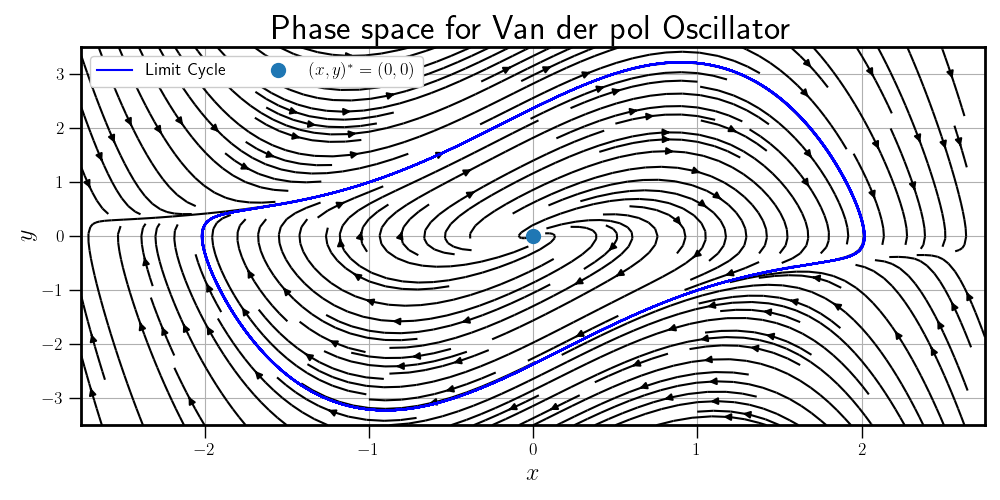
\includegraphics[width=\textwidth]{../Figures/van_der_pol_phase_space.png}
        \end{figure}
    \end{frame}

    \begin{frame}
        \frametitle{Results - Van der Pol loss curves and phase space}
        \begin{figure}
            \centering
            \begin{minipage}{.5\textwidth}
                \includegraphics[width=\textwidth]{"Z:/ML_models/DLDMD-newest/examples/van_der_pol/loss_plots_square.png"}
            \end{minipage}%
            \begin{minipage}{.5\textwidth}
                \includegraphics[width=\textwidth]{"Z:/ML_models/DLDMD-newest/examples/van_der_pol/experiment_trajectories.png"}
            \end{minipage}
        \end{figure}
    \end{frame}

    \begin{frame}
        \frametitle{Results - Van der Pol linear fit slopes} 
        \begin{figure}
            \centering
            \begin{minipage}{.3333\textwidth}
                \includegraphics[width=\textwidth]{"Z:/ML_models/DLDMD-newest/examples/van_der_pol/slope_linear_fit_enc_in_square.png"}
                \includegraphics[width=\textwidth]{"Z:/ML_models/DLDMD-newest/examples/van_der_pol/slope_linear_fit_enc_2_square.png"}
                \includegraphics[width=\textwidth]{"Z:/ML_models/DLDMD-newest/examples/van_der_pol/slope_linear_fit_dec_0_square.png"}
            \end{minipage}%
            \begin{minipage}{.3333\textwidth}
                \includegraphics[width=\textwidth]{"Z:/ML_models/DLDMD-newest/examples/van_der_pol/slope_linear_fit_enc_0_square.png"}
                \includegraphics[width=\textwidth]{"Z:/ML_models/DLDMD-newest/examples/van_der_pol/slope_linear_fit_enc_out_square.png"}
                \includegraphics[width=\textwidth]{"Z:/ML_models/DLDMD-newest/examples/van_der_pol/slope_linear_fit_dec_1_square.png"}
            \end{minipage}%
            \begin{minipage}{.3333\textwidth}
                \includegraphics[width=\textwidth]{"Z:/ML_models/DLDMD-newest/examples/van_der_pol/slope_linear_fit_enc_1_square.png"}
                \includegraphics[width=\textwidth]{"Z:/ML_models/DLDMD-newest/examples/van_der_pol/slope_linear_fit_dec_in_square.png"}
                \includegraphics[width=\textwidth]{"Z:/ML_models/DLDMD-newest/examples/van_der_pol/slope_linear_fit_dec_2_square.png"}
            \end{minipage}
            \includegraphics[width=.3333\textwidth]{"Z:/ML_models/DLDMD-newest/examples/van_der_pol/slope_linear_fit_dec_out_square.png"}
        \end{figure}
    \end{frame}

    \begin{frame}
        \frametitle{Results - Van der Pol linear fit slope averages and variances}
        
        \begin{figure}
            \centering
            \includegraphics[width=\textwidth]{"Z:/ML_models/DLDMD-newest/examples/van_der_pol/slope_linear_fit.png"}
        \end{figure}
    \end{frame}

    \begin{frame}
        \frametitle{Results - Van der Pol notes}

    \end{frame}

\end{document}